  %  \nonstopmode
  % !TEX encoding = UTF-8 Unicode
\documentclass[10pt,letterpaper,cm]{nupset}
\usepackage[margin=1in]{geometry}
\usepackage[utf8]{inputenc}
\usepackage[T1]{fontenc}
\usepackage{graphicx}
\usepackage{enumerate}
\usepackage{enumitem}
\usepackage{float}
\usepackage{stmaryrd}
\usepackage{amsfonts}
\usepackage{amssymb}
\usepackage{mathtools}
\usepackage{upgreek}
\usepackage{pgfplots}
\pgfplotsset{compat=1.13}
\usepackage{amsmath,amsthm}
\usepackage{tikz-cd}
\usetikzlibrary{trees}
\usetikzlibrary{knots,calc}
\usepackage{xcolor}
\usepackage{soul}
\usetikzlibrary{decorations.markings}
\usepackage{faktor}
\usepackage{xfrac}
\usepackage{ mathrsfs }
\usepackage{hyperref}
\usepackage{comment}
\usepackage[linesnumbered,ruled]{algorithm2e}
\hypersetup{colorlinks=true, linkcolor=red,          % color of internal links (change box color with linkbordercolor)
    citecolor=green,        % color of links to bibliography
    filecolor=magenta,      % color of file links
    urlcolor=cyan           }
\usepackage{adjustbox}
\usepackage{media9}


\usepackage{thmtools}
\usepackage[capitalise]{cleveref} 
    
\theoremstyle{definition}
\newtheorem{definition}{Definition}
\newtheorem{exmp}[definition]{Example}
\newtheorem{non-exmp}[definition]{Non-example}
\newtheorem{note}[definition]{Note}

\theoremstyle{theorem}
\newtheorem{theorem}[definition]{Theorem}
\newtheorem{lemma}[definition]{Lemma}
\newtheorem{prop}[definition]{Proposition}
\newtheorem{corollary}[definition]{Corollary}
\newtheorem{claim}{Claim}
\newtheorem{exercise}[definition]{Exercise}

\theoremstyle{remark}
\newtheorem*{remark}{Remark}
\newtheorem*{todo}{To do}
\newtheorem*{question}{Question}
\newtheorem*{conv}{Convention}
\newtheorem*{aside}{Aside}
\newtheorem*{notation}{Notation}
\newtheorem*{term}{Terminology}
\newtheorem*{background}{Background}
\newtheorem*{further}{Further reading}
\newtheorem*{sources}{Sources}

\makeatletter
\def\th@plain{%
  \thm@notefont{}% same as heading font
  \itshape % body font
}
\def\th@definition{%
  \thm@notefont{}% same as heading font
  \normalfont % body font
}
\makeatother


\makeatletter
\renewcommand*\env@matrix[1][*\c@MaxMatrixCols c]{%
  \hskip -\arraycolsep
  \let\@ifnextchar\new@ifnextchar
  \array{#1}}
\makeatother
\pgfplotsset{unit circle/.style={width=4cm,height=4cm,axis lines=middle,xtick=\empty,ytick=\empty,axis equal,enlargelimits,xmax=1,ymax=1,xmin=-1,ymin=-1,domain=0:pi/2}}
\DeclareMathOperator{\Ima}{Im}
\newcommand{\A}{\mathbb A}
\newcommand{\C}{\mathbb C}
\newcommand{\D}{\mathbb D}
\newcommand{\E}{\mathbb E}
\newcommand{\CP}{\mathbb{CP}}
\newcommand{\F}{\mathbb F}
\newcommand{\G}{\vec G}
\renewcommand{\H}{\mathbb H}
\newcommand{\HP}{\mathbb HP}
\newcommand{\K}{\mathbb K}
\newcommand{\M}{\mathbb M}
\renewcommand{\L}{\mathcal L}
\newcommand{\N}{\mathbb N}
\renewcommand{\O}{\mathbf O}
\newcommand{\OP}{\mathbb OP}
\renewcommand{\P}{\mathcal P}
\newcommand{\Q}{\mathbb Q}
\newcommand{\U}{\mathcal U}
\newcommand{\I}{\mathbb I}
\newcommand{\R}{\mathbb{R}}
\newcommand{\RP}{\mathbb{RP}}
\renewcommand{\S}{\mathbb S}
\newcommand{\T}{\mathcal T}
\newcommand{\X}{\mathbf X}
\newcommand{\Z}{\mathbb Z}
\newcommand{\B}{\mathbb{B}}
\newcommand{\TM}{\mathsf{TM}}
\newcommand{\1}{\mathbb{1}}
\newcommand{\ds}{\displaystyle}
\newcommand{\ran}{\right>}
\newcommand{\lan}{\left<}
\newcommand{\bmat}[1]{\begin{bmatrix} #1 \end{bmatrix}}
\renewcommand{\a}{\vec{a}}
\renewcommand{\b}{\vec b}
\renewcommand{\c}{\vec c}
\renewcommand{\d}{\vec d}
\newcommand{\e}{\vec e}
\newcommand{\h}{\vec h}
\newcommand{\f}{\vec f}
\newcommand{\g}{\vec g}
\renewcommand{\i}{\vec i}
\renewcommand{\j}{\vec j}
\renewcommand{\k}{\vec k}
\newcommand{\n}{\vec n}
\newcommand{\p}{\vec p}
\newcommand{\q}{\vec q}
\renewcommand{\r}{\vec r}
\newcommand{\s}{\vec s}
\renewcommand{\t}{\vec t}
\renewcommand{\u}{\vec u}
\newcommand{\w}{\vec w}
\newcommand{\x}{\vec x}
\newcommand{\y}{\vec y}
\newcommand{\z}{\vec z}
\newcommand{\0}{\vec 0}
\newcommand{\pt}{\mathsf{pt}}
\newcommand{\from}{\longleftarrow}
\newcommand{\intprodl}{%
    \mathbin{\scalebox{1.5}{$\lrcorner$}}%
}
\newcommand{\intprodr}{%
    \mathbin{\scalebox{1.5}{$\llcorner$}}%
}
\DeclareMathOperator*{\Span}{span}
\DeclareMathOperator{\rng}{range}
\DeclareMathOperator{\gemu}{gemu}
\DeclareMathOperator{\almu}{almu}
\newcommand{\Char}{\mathsf{char}}
\DeclareMathOperator{\id}{id}
\DeclareMathOperator{\tr}{Tr}
\DeclareMathOperator{\tor}{Tor}
\DeclareMathOperator{\im}{im}
\DeclareMathOperator{\homeo}{Homeo}
\DeclareMathOperator{\GL}{GL}
\DeclareMathOperator{\SL}{SL}
\DeclareMathOperator{\norm}{N}
\DeclareMathOperator{\aut}{Aut}
\DeclareMathOperator{\Int}{Int}
\DeclareMathOperator{\ext}{Ext}
\DeclareMathOperator{\supp}{supp}
\DeclareMathOperator{\cl}{cl}
\DeclareMathOperator{\dom}{dom}
\DeclareMathOperator{\rnk}{rank}
\DeclareMathOperator{\Hom}{Hom}
\DeclareMathOperator{\Alt}{Alt}
\DeclareMathOperator{\dr}{dR}
\DeclareMathOperator{\ed}{End}
\DeclareMathOperator{\BM}{BM}
\DeclareMathOperator{\ob}{ob}
\DeclareMathOperator{\clength}{cup{-}length}
\DeclareMathOperator{\sgn}{sgn}
\DeclareMathOperator{\orb}{Orb}
\DeclareMathOperator{\cyl}{Cyl}
\DeclareMathOperator{\rel}{rel}
\DeclareMathOperator{\res}{res}
\DeclareMathOperator{\cat}{cat}
\DeclareMathOperator{\op}{op}
\DeclareMathOperator{\Gd}{Gd}
\DeclareMathOperator{\coker}{coker}
\DeclareMathOperator{\map}{Map}
\DeclareMathOperator{\sing}{Sing}
\DeclareMathOperator{\Op}{\mathbf{Op}}
\DeclareMathOperator{\colim}{colim}
\DeclareMathOperator{\tot}{Tot}
\DeclareMathOperator{\ef}{EF}
\DeclareMathOperator{\thh}{\mathsf{Th}}
\DeclareMathOperator{\cn}{\mathsf{Cn}}
\DeclareMathOperator{\pgl}{PGL}
\DeclareMathOperator{\fo}{\mathsf{FO}}
\DeclareMathOperator{\Et}{\acute{E}t}
\DeclareMathOperator{\ch}{\mathbf{Ch}}
\DeclareMathOperator{\vf}{\mathscr{X}}

\newcommand{\bi}{\begin{itemize}}
\newcommand{\ei}{\end{itemize}}

\newcommand{\be}{\begin{enumerate}}
\newcommand{\ee}{\end{enumerate}}

\newcommand{\bmp}{\begin{mathpar}}
\newcommand{\emp}{\end{mathpar}}

\setlength{\parindent}{0pt}

\newcommand{\mathcolorbox}[2]{\colorbox{#1}{$\displaystyle #2$}}

\newlist{steps}{enumerate}{1}
\setlist[steps, 1]{label = Step \arabic*:}

% info for header block in upper right hand corner
\name{Perry Hart}
\class{MATH 571}
\assignment{Spring 2020}

\begin{document}

\begin{abstract}
We present solutions to all exercises from Scott Weinstein's ``Model Theory'' course lectures at UPenn. These are largely self-contained and are meant to complement Weinstein's written memoirs of our class meetings. The official reference for the course is David Marker's \textit{Model Theory: An Introduction}.
\end{abstract}

\begin{problem}[1.] 
Let $I$ be a countably infinite set. Let $\D \coloneqq \left\langle I, E\right\rangle$ be a structure where $E$ is an equivalence relation for which  there is exactly one equivalence class of size $k$ for each $k\in \Z_{\geq 1}$.
\be[label=(\arabic*)]
\item Show that the set $\Lambda$ of (first-order) sentences expressing that $E$ is an equivalence relation with exactly one equivalence class of size $k$ for each $k\in \Z_{\geq 1}$ axiomatizes $\D$, i.e., $\thh(\D) = \cn(\Lambda)$ where 
\[
\cn(\Lambda) \coloneqq  \left\{\varphi \in \fo_{\D} \mid \Lambda \models \varphi\right\}
.\]
\item Show that for every (first-order) formula $\theta(y, \overline{w})$ and every $\bar{a}\in I$, the set $$\theta\left[\D, \bar{a}\right] \coloneqq \left\{x\in \dom(\D) \mid \D\models \theta\left[x, \bar{a}\right]\right\}$$ is either finite or cofinite.
\ee
\end{problem}
\begin{solution} $ $
\be[label=(\arabic*)]
\item It suffices to prove that $\Lambda$ is complete. For, in this case, any two models of $\Lambda$ must be elementarily equivalent.
\begin{claim}\label{C1}
Let $\E$ be any model of $\Lambda$ of size $\kappa \geq \omega$. There exists an elementary extension $\E_{\kappa} \succeq \E$ of size $\kappa$ such that $\E_{\kappa}$ has exactly $\kappa$ equivalence classes each of size $\kappa$.
\end{claim} 
\begin{proof}
Let $\lambda$ denote the cardinality of the set of all equivalence classes in $\dom(\E)$. Note that $\lambda \leq \kappa$. For every $\alpha,\beta \in \kappa$, adjoin to the language of $\E$ a new constant symbol $c(\alpha, \beta)$. Consider the theory
\[
\Delta \coloneqq \Lambda   \cup \left\{E{c(x,y)}{c(x,z)} \mid x,y,z \in \kappa \right\} \cup \left\{ \neg{E{c(x,0)}{c(y,0)}} \mid x,y\in \kappa, \ x\ne y\right\} .
\]
Any finite subset $F$ of $\Delta$ is satisfiable by a suitable expansion $\E_F$ of $\E$. Then there exists an ultrafilter on the family of finite subsets of $\Delta$ such that the ultraproduct $$\prod_{\underset{\text{finite}}{F\subset \Delta}}\E_F/\mathcal{U}$$ satisfies $\Delta$. Moreover, its reduct $\A$ to the language of $\E$ is an elementary extension of $\E$. By the downward L\"owenheim-Skolem theorem, there exists a structure $\E_0$ of size $\kappa$ such that $\A \succeq \E_0 \succeq \E$.

Now, repeat our preceding construction $\omega$ times to get an increasing chain
\[
\E \preceq \E_0 \preceq \E_1 \preceq  \E_2 \preceq \cdots
\]
of structures such that each $\dom(\E_i)$ has cardinality $\kappa$. Note that $\E_{\kappa}$ is an elementary extension of $\E$. Further, the domain of the direct limit $\E_{\kappa} \coloneqq \bigcup_{i\in \omega}\E_i$ also has cardinality $\kappa$, so that $\E_{\kappa}$ has exactly $\kappa$ equivalence classes. Finally, for any $x\in \E_{\kappa}$, $x$ belongs to some $\E_n$. Hence the equivalence class $\left[x\right]$ has size $\kappa$ in $\E_{n+1}$ and thus in $\E_{\kappa}$. It follows that every equivalence class in $\E_{\kappa}$ has size $\kappa$.
\end{proof}

Suppose, toward a contradiction, that there is a sentence $\varphi$ in the language of $\D$ such that neither $\varphi$ nor $\neg{\varphi}$ belongs to  $\cn(\Lambda)$. Then there are models $\A^1$ and $\A^2$ of $\Lambda$ a such that $\A^1 \models \neg{\varphi}$ and $\A^2 \models \varphi$. By the L\"owenheim-Skolem theorem, we may assume that both of these have size $\kappa \geq \omega$. By \cref{C1}, we thus have two  structures $\A^1_{\kappa}$ and $\A^2_{\kappa}$ such that $\A^1_{\kappa} \models \neg{\varphi}$ and $\A^2_{\kappa}\models \varphi$. But it's easy to see that $\A^1_{\kappa}$ and $\A^2_{\kappa}$ must be isomorphic, which yields a contradiction.
\item Suppose, toward a contradiction, that there exist a formula $\theta(y, w_1, \ldots, w_n)$ and an element $\bar{a}\in I$ such that $\theta\left[\D, \bar{a}\right]$ is both infinite and coinfinite. Adjoin to the language of $\D$ new constant symbols $\bar{e} \coloneqq \left(e_1, \ldots, e_n\right)$, $c$, and $d$. For each $k\in \Z_{\geq 1}$, let $\lambda_k(x)$ denote the formula expressing that the equivalence class of $x$ has cardinality $>k$. Now, consider the theory
\begin{align*}
\Gamma \coloneqq \Lambda  \cup \left\{\lambda_k(c) \mid k \geq 1\right\} & \cup \left\{\lambda_k(d) \mid k \geq 1\right\} 
\\ & \cup \left\{\neg{E{e_i}{c}} \mid 1\leq i \leq n\right\} 
\\ & \cup \left\{\neg{E{e_i}{d}} \mid 1\leq i \leq n\right\} 
\\ & \cup \left\{\theta(c, \bar{e}), \neg{\theta(d, \bar{e})}\right\}
\end{align*}
in our new language.

Let $F$ be any finite subset of $\Gamma$. Since both $\theta\left[\D, \bar{a}\right]$ and $\neg{\theta\left[\D, \bar{a}\right]}$ are infinite by assumption, we can find an expansion of $\D$ that satisfies $F$ by interpreting $\bar{e}$ as $\bar{a}$ and both $c$ and $d$ as members of large enough equivalence classes. By the compactness theorem, it follows that there is some model $\C$ of $\Gamma$, which must be infinite. Let $\C'$ denote the reduct of $\C$ to the language of $\D$. Thanks to the L\"owenheim-Skolem theorem, we may assume that $\dom(\C')$ is countable. Thus, the equivalence classes $\left[c^{\C}\right]$ and $\left[d^{\C}\right]$ are countable. Note that $e_i^{\C} \notin \left[c^{\C}\right] \cup \left[d^{\C}\right]$ for each $1\leq i \leq n$. Therefore, there is an automorphism of $\C'$ sending $c^{\C}$ to $d^{\C}$ and fixing each $e_i^{\C}$. But this contradicts the fact that $\C' \models \theta\left[c^{\C}, \bar{e}^{\C}\right] \land \neg{\theta\left[d^{\C}, \bar{e}^{\C}\right]}$.
\ee
\end{solution}

\medskip

\begin{definition}[Categoricity]
For any cardinal $\kappa$, we say that a theory $T$ is \textit{$\kappa$-categorical} if any two models of $T$ of size $\kappa$ are isomorphic.
\end{definition}

\begin{problem}[2.]
Show that a $\L$-structure $\A$ is finite if and only if for any $\L$-structure $\B$,
\[ \A \equiv \B \iff \A \cong \B.\]
\begin{remark}
This shows that any complete theory with a finite model is $\kappa$-categorical for \emph{any} cardinal $\kappa$.
\end{remark}
\end{problem}
\begin{solution}

$(\Longrightarrow)$

\smallskip

It is always true that any two isomorphic structures are elementarily equivalent. Thus, it remains to show that $\A \equiv \B \implies \A \cong \B$.

\smallskip

First, assume that $\L$ is finite. Consider the \textit{atomic diagram} of $\A$, i.e., the set $$\mathtt{D}(\A)\coloneqq \left\{\varphi \mid \underline{\A} \models \varphi, \  \varphi \text{ is either atomic or the negation of an atomic formula}\right\}$$ where $\underline{\A}$ denotes the expansion of $\A$ obtained by adjoining a constant symbol $c_a$ for each $a\in \dom(\A)$. Since both $\L$ and $\dom(\A)$ are finite, we can encode $\mathtt{D}(\A)$ with a single sentence $\psi$. Therefore, the sentence $$\psi_{\A} \coloneqq \forall{x}\left(\bigvee_{a\in \dom(\A)} x=c_a\right) \land \psi$$ has the property that $\underline{\B} \models \psi_{\A} \implies \B \cong \A$ for any other $\L$-structure $\B$. Now, if $\A \equiv \B$, then clearly both $\underline{\A}$ and $\underline{\B}$ satisfy $\psi_{\A}$, so that $\B \cong \A$.

\smallskip

Next, let $\L$ be arbitrary and let $\A \equiv \B$. Suppose, toward a contradiction, that $\A \not\cong \B$. Then for any bijection $f: \dom(\A) \to \dom(\B)$, there is some finite sublanguage $\L_f$ of $\L$ such that $f$ is \emph{not} an isomorphism $\A^{\L_f}\to \B^{\L_f}$ of reducts to $\L_f$. Consider the language $$\L' \coloneqq \bigcup_{\underset{\text{bijection}}{f:\dom(\A)\to \dom(\B)}}\L_f,$$ which is finite as the finite union of finite sets. Thanks to our preceding discussion, we obtain an isomorphism $g: \A^{\L'}\overset{\cong}{\longrightarrow} \B^{\L'}$. But $\L_g \subset \L'$ by our construction of $\L'$, and thus $g$ induces an isomorphism $\A^{\L_g}\overset{\cong}{\longrightarrow} \B^{\L_g}$, contrary to our choice of $\L_g$.

\medskip

$(\Longleftarrow)$

\smallskip

Suppose that $\A$ is infinite. We must find a structure $\B$ such that $\A \equiv \B$ but $\A \not\cong \B$. But this follows at once from the the L\"owenheim-Skolem theorem, which implies that $\thh(\A)$ has a model of any infinite size. 

\end{solution}

\medskip

\begin{definition}[Ehrenfeucht-Fra\"{\i}ss\'e  game]
Suppose that $\L$ is a finite language without function symbols. Let $\D$ and $\E$ be two $\L$-structures. Let $n\in \omega$. The \textit{Ehrenfeucht-Fra\"{\i}ss\'e  game $\ef_n(\D, \E)$ of length $n$ on $\D$ and $\E$} is a game of perfect information played as follows.
\begin{enumerate}[label=(\alph*)]
\item There are exactly two players, the \textit{spoiler} and the \textit{duplicator}.
\item There are exactly $n$ rounds.
\item The spoiler begins round $k\leq n$ by picking an element (sometimes called a pebble) of either $\dom(\D)$ or $\dom(\E)$. Next, the duplicator picks an element of the other domain.
\item This yields two sequences $\left(d_1, \ldots, d_n\right)$ and $\left(e_1, \ldots, e_n\right)$ such that $d_i\in \dom(\D)$ and $e_i\in \dom(\E)$ for each $i=1, \ldots, n$.  If the mapping $d_i \mapsto e_i$ defines an isomorphism of finite substructures, then we say that the duplicator has won $\ef_n(\D, \E)$. Otherwise, we say that the spoiler has won.
\end{enumerate}
\end{definition}

\begin{theorem}[Fra\"{\i}ss\'e]\label{EF}
The duplicator has a winning strategy in $\ef_n(\D, \E)$ for each $n\in \omega$ if and only if $\D \equiv \E$.
\end{theorem}

\begin{problem}[3.]
Let $\N^{\ast} = \left\langle \omega, <\right\rangle$. Show that for any infinite cardinal $\kappa$, $\thh(\N^{\ast})$ is \emph{not} $\kappa$-categorical.
\end{problem}
\begin{solution}
Expand the language of $\N^{\ast}$ by adjoining countably many constants $\left\{c_i\right\}_{i\in \Z}$. Consider the theory
\[ \label{eqn:st1}
T \coloneqq \thh(\N^{\ast}) \cup \left\{ c_i > c_{i+1} \mid i\in \Z \right\}. \tag{$\star$}
\] in our new language.  Any finite subset of $T$ is satisfied by an expansion of $\N^{\ast}$ suitably interpreting the $c_i$ since $\N^{\ast}$ has descending chains of all finite lengths. By the compactness theorem, it follows that there is some model $\A$ of $T$, which must be infinite. If $\left\lvert{\A}\right\rvert >\aleph_0$, then apply the L\"owenheim-Skolem theorem to get a model $\B$ of $T$ such that $\left\lvert{\B}\right\rvert = \aleph_0$.  Let 
\[
\A' = \begin{cases} \B & \left\lvert{\A}\right\rvert >\aleph_0
\\ \A & \left\lvert{\A}\right\rvert =\aleph_0
\end{cases}.
\] Note that $\A' \models T$. Since the property of being a linearly ordered set is expressible by a first-order sentence, we see that $\A'$ is linearly ordered by $<$. Further, we see that $\A'$ has an infinite descending chain, which means that $\A'$ is not well-ordered by $<$.  But $\left(\omega, <\right)$ is a well-ordered set, and thus the reduct of $\A'$ to the language of $\N^{\ast}$ is not isomorphic to $\N^{\ast}$. It does, however, satisfy $\thh(\N^{\ast})$. This shows that $\thh(\N^{\ast})$ is not $\aleph_0$-categorical.

\medskip

Unfortunately, it's unclear that this method can be adapted to show that $\thh(\N^{\ast})$ is not $\kappa$-categorical when $\kappa$ is uncountable. In this case, we instead shall employ two binary  operations on the class of all linear orderings.
Let $L_1$ and $L_2$ be linearly ordered sets.
\begin{itemize}
\item $L_1^{\op}$ refers to $L_1$ equipped with the inverse order.
\item $L_1 \otimes L_2$ refers to $L_1 \times L_2$ equipped with the lexicographic order.
\item ${L_1 \oplus L_2}$ refers to $L_1$ with its ordering followed by $L_2$ with its ordering.
\end{itemize}
Now, consider the following linearly ordered structures:
\begin{gather*}
 {\N^{\ast} \oplus \left(\Z \otimes\kappa\right)}
\\ {\N^{\ast}  \oplus  \left(\Z \otimes\left(\Q  \oplus\kappa\right)\right)},
\end{gather*} both of which have cardinality $\kappa$.
These orderings possess bottom elements and are \textit{discrete} in the sense that both structures satisfy the sentences
\begin{align}
\begin{split}
& \forall{x}\exists{y}\left(x<y \land \neg{\exists{z}\left(x<z \land z<y\right)}\right) \\
 \forall{x}&\left(\exists{w}\left(w < x\right)\rightarrow \exists{y}\left(y<x \land \neg{\exists{z}\left(y<z \land z<x\right)}\right)\right).
\end{split} \label{eqn:disc}
\end{align}
(Informally, we can view $y$ here as the \textit{successor}/\textit{predecessor} of $x$.) Note that, on the one hand, $ {\N^{\ast}  \oplus \left(\Z \otimes\kappa\right)}$ cannot possess an descending chain of length $\omega^2$, for otherwise $\kappa$, which is well-ordered, would possess an infinite descending chain. On the other hand, ${\N^{\ast}  \oplus  \left(\Z \otimes\left(\Q  \oplus \kappa\right)\right)}$ does possess such a chain since $\omega^{\ast}$ (the order type of $\Z_{<0}$) can be embedded in $\Q$. Therefore, \[
{\N^{\ast}  \oplus \left(\Z \otimes\kappa\right)} \not\cong {\N^{\ast}  \oplus  \left(\Z \otimes\left(\Q  \oplus\kappa\right)\right)}.
\]

\begin{claim}
Suppose that $\left(\E, <\right)$ is a discrete linear ordering with a bottom element but no top element. Then $\E \equiv \N^{\ast}$.
\end{claim}
\begin{proof}[Proof sketch]
Consider the Ehrenfeucht-Fra\"{\i}ss\'e  game $\ef_n(\E, \N^{\ast})$. The duplicator has a winning strategy in $\ef_n(\E, \N^{\ast})$ by adhering to the following rules.
\begin{enumerate}[label=(\roman*)]
\item If, in round $m$, the spoiler chooses an element of one of the structures that is connected to a previously chosen element or the bottom element by a path of successors of length $k<\infty$, then choose the corresponding element of the other structure in round $m$.
\item Otherwise, make sure that any chosen element of $\dom(\N^{\ast})$ is always separated by at least $n+1$ elements from any previously chosen element of $\dom(\N^{\ast})$ while preserving the required order of your choices. 

In this case, choose first a natural number separated by more than $3^n$ elements from the greatest previously chosen clement of $\dom(\N^{\ast})$.
\end{enumerate}
\end{proof}
Thanks to \cref{EF}, it follows that both $ {\N^{\ast}  \oplus \left(\Z \otimes\kappa\right)}$ and ${\N^{\ast}  \oplus  \left(\Z \otimes\left(\Q  \oplus\kappa\right)\right)}$ are elementarily equivalent to $\N^{\ast}$ and thus models of $\thh(\N^{\ast})$. Hence $\thh(\N^{\ast})$ is not $\kappa$-categorical. 
\end{solution}

\begin{problem}[4.]
Show that any set definable over $\N^{\ast}$ is either finite or cofinite. 
\begin{remark}
This shows that $\N^{\ast}$ is \textit{o-minimal} in the sense that every definable set over $\N^{\ast}$ is a finite union of points and intervals in $\omega$. 
\end{remark}
\end{problem}
\begin{solution}
Note that any set definable over $\N^{\ast}$ is $0$-definable  because any natural number $n$ is uniquely determined by the first-order property
\[
\begin{cases}
 ``n \text{ is less than any other element}" & n=0
\\``\text{there are exactly }n-1\text{ elements between $0$ (the bottom element) and }n"  & n>1
\end{cases}.
\]
Suppose, toward a contradiction, that there exist a formula $\theta(y)$ such that $\theta\left[\N^{\ast}\right]$ is both infinite and coinfinite. Consider, again, the theory \eqref{eqn:st1}. Let $$T' = T \cup \left\{\theta(c_0), \neg{\theta(c_1)}\right\}.$$ Since both $\theta\left[\N^{\ast}\right]$ and $\neg{\theta\left[\N^{\ast}\right]}$ are infinite by assumption, we can find an expansion of $\N^{\ast}$ that satisfies any finite subset of $T'$, By the compactness theorem together with the L\"owenheim-Skolem theorem, we thus can find a countable model $\D$ of $T'$ and take its reduct $\C$ to the language of $\N^{\ast}$. Note that $\left(\dom(\C), < \right)$ is a countable linear ordering with an  infinite descending and ascending chain $\chi$ on which both $c_0^{\D}$ and $c_1^{\D}$ lie. Moreover, this ordering is discrete in the sense of \eqref{eqn:disc}.
Therefore, we may assume that $\chi$ has the form
\[
 \cdots < x_{m-1} < x_m < x_{m+1} < \cdots
\] where $x_{m+1}$ denotes the immediate successor of $x_m$. There is an automorphism of $\C$ mapping $c_0^{\D}$ to $c_1^{\D}$ by suitably shifting $\chi$ finitely many places to the left and fixing all elements outside $\chi$. But this contradicts the fact that $\C \models \theta\left[c_0^{\D}\right] \land \neg{\theta\left[c_1^{\D}\right]}$.
\end{solution}

\begin{problem}[5.]
Consider the theory $\mathsf{DLO}$ of the dense linear ordering without endpoints. For any uncountable cardinal $\kappa$, show that there are $2^{\kappa}$ many models of $\mathsf{DLO}$ up to isomorphism.
\begin{remark}
This shows that $\mathsf{DLO}$ is \emph{not} $\kappa$-categorical even though it is $\aleph_0$-categorical.
\end{remark}
\end{problem}
\begin{solution}
Consider the linear orderings 
\begin{gather*}
L_1 \coloneqq \Q \otimes\left(\omega_1^{\op}  \oplus \omega_1  \right)
\\ L_2\coloneqq  \Q \otimes\left(1 \oplus \omega_1^{\op}  \oplus \omega_1 \right).
\end{gather*}
Now, by replacing each $\alpha \in \kappa$ with a choice of $L_1$ or $L_2$, we obtain $2^{\kappa}$ many dense linear orderings $\left\{P_{\beta}\right\}_{\beta< 2^{\kappa}}$ without endpoints such that $\left\lvert{P_{\beta}}\right\rvert=\kappa$ for ever $\beta$. It remains to show that these are pairwise non-isomorphic.

\smallskip

To this end, suppose that there is an isomorphism $f: P_{\beta} \overset{\cong}{\longrightarrow} P_{\beta'}$. By construction, both $P_{\beta}$ and $P_{\beta'}$ consist of $\kappa$-sequences 
\begin{align*}
L_{i_0} & < L_{i_1} < \cdots < L_{i_{\alpha}} < \cdots
\\ L_{i_0'} & < L_{i_1'} < \cdots < L_{i_{\alpha}'} < \cdots, 
\end{align*}
respectively, where $i_{\alpha}, i_{\alpha}'\in \left\{1,2\right\}$ Since any isomorphism of well-ordered sets is unique, we see that the function $f\restriction_{L_{i_{\alpha}}}$ is an isomorphism $L_{i_{\alpha}} \overset{\cong}{\longrightarrow} L_{i_{\alpha}'}$ for any $\alpha \in \kappa$.

\begin{claim}
$L_1 \not\cong L_2$.
\end{claim}
\begin{proof}
On the one hand,  $L_1$ has a suborder isomorphic to $\omega_1^{\op}$ with no lower bound in $L_1$. On the other hand, any such suborder of $L_2$ has a lower bound in $L_2$. Hence there is no isomorphism from $L_1$ to $L_2$.
\end{proof}

It follows that $L_{i_{\alpha}} = L_{i_{\alpha}'}$ for every $\alpha \in \kappa$, which completes our proof.

\begin{comment}
\begin{definition} Let $\left(L, \leq \right)$ be any linear order and let $C\coloneqq \left(X, Y\right)$ be any (Dedekind) cut in $L$. Let   $\lambda$ and $\lambda'$ be cardinals.
\begin{enumerate}
\item We say that $C$ is \textit{filled} if there exists $s\in Y$ such that $s\leq y$ for any $y\in Y$.

Otherwise, we say that $C$ is \textit{unfilled}.
\item If $C$ is unfilled, then $C$ has \textit{cofinality type $\left(\lambda, \lambda'\right)$} if the length of the shortest increasing sequence unbounded in $X$ is $\lambda$ and the length of the shortest decreasing sequence unbounded in $Y$ is $\lambda'$.

If $C$ is filled by $s\in Y$, then $C$ has \textit{cofinality type $\left(\lambda, \lambda'\right)$} if the length of the shortest increasing sequence unbounded in $X$ is $\lambda$ and the length of the shortest decreasing sequence in $Y$ converging to $s$ is $\lambda'$.
\end{enumerate} 
\end{definition}
Now, $f$ induces a bijection $\hat{f}$ from the set $S_{\beta}$ of cuts  in $P_{\beta} $ with cofinality type $\left(\aleph_1, \aleph_1\right)$
to the set $S_{\beta'}$ of such cuts in $P_{\beta'}$. Note that both $S_{\beta}$ and $S_{\beta'}$ inherit well-orderings from $\kappa$, so that $\hat{f}$ is actually an order isomorphism. Since any isomorphism of well-ordered sets is unique, we see that for each $\gamma \in \kappa_{\geq 1}$, $\hat{f}$ sends any  cut of the form
\[\label{eqn:one}
\left(\bigcup_{\alpha < \gamma}L_{i_{\alpha}}, \bigcup_{\alpha \geq  \gamma}L_{i_{\alpha}}\right), \ \quad i_{\alpha}\in \left\{1,2\right\} \tag{1}
\]
to another cut of the form
\[\label{eqn:two}
\left(\bigcup_{\alpha < \gamma}L_{i_{\alpha}'}, \bigcup_{\alpha \geq \gamma}L_{i_{\alpha}'}\right), \ \quad i_{\alpha}'\in \left\{1,2\right\}. \tag{2}
\]
Moreover, since $\hat{f}$ is an isomorphism, \eqref{eqn:one} is filled if and only if \eqref{eqn:two} is filled. 
\end{comment}

\end{solution}

\medskip

\begin{definition}
Let $T$ be a theory and let $\Gamma(\bar{x})$ be a set of formulas in free variables $x_1, \ldots, x_n$. We say that $\Gamma$ is an \textit{$n$-type over $T$} if for any finite subset $\Delta \subset \Gamma$, the expanded theory $$T\cup \left\{\left(\exists{\bar{x}}\right)\bigwedge{\Delta}\right\}$$ is satisfiable.
\end{definition}

\begin{notation}
Let $\M$ be an $\L$-structure and let $A\subset \dom(\M)$. Let $\L_A = \L \cup \left\{c_a \mid a \in A\right\}$ and let $\M_A$ denote the  $\L_A$-structure induced by $\M$.  Then  $\S_n^{\M}(A)$ refers to the set of all complete $n$-types over $\thh_A(\M) \coloneqq \thh(\M_A)$.
\end{notation}
\begin{definition}[Stability] Let $T$ be a complete theory in $\L$ and let $\kappa$ be an infinite cardinal.  
\begin{comment}
\begin{enumerate}[label=(\roman*)]
\item Let $p$ be the set of all $\L_A$ formulas in free variables $x_1, \ldots, x_n$. We say that $p$ is \textit{$n$-type} if $p \cup \thh_A(\M)$ is satisfiable.

In this case, we call $p$ \textit{complete} if $\theta \in p$ or $\neg{\theta}$ for any $\L_A$-formula $\theta$ with free variables among $x_1, \ldots, x_n$. 
\item
\end{enumerate}
\end{comment}
We say that $T$ is \textit{$\kappa$-stable} if whenever $\M \models T$, $A\subset \dom(\M)$, and $\left\lvert{A}\right\rvert = \kappa$, we have that $\left\lvert{\S_n^{\M}(A)}\right\rvert = \kappa$.
\end{definition} 

\pagebreak

\begin{problem}[6.]
Let $\A$ be a structure and $\theta(x,y)$ be a formula in the language of $\A$. Suppose that $B\subset \dom(\A)$ is an infinite set on which $\theta[\A]$ is a linear order $\prec$. 
Show that $\thh(\A)$ is \emph{not} $\omega$-stable (i.e., $\aleph_0$-stable).
\end{problem}
\begin{solution}
Thanks to the axiom of dependent choice, we can find a countably infinite chain of at least one of the following two forms.
\begin{align*}
a_0 &\prec b_0\prec a_1 \prec b_1 \prec a_2 \prec b_2 \prec\cdots
\\ \cdots &\prec b_2 \prec a_2 \prec b_1 \prec a_1 \prec b_0 \prec a_0
\end{align*}   with $a_i, b_i\in B$ for each $i=0,1,2,\ldots$. Without loss of generality, assume that we can find the former kind of chain and that $\theta$ has the form $x\prec y$. In this case, 
\[ \label{eqn:order}
\A \models \theta[a_i, b_j] \iff i\leq j. \tag{$\ast$}
\] 

\begin{claim}
There exist sequences $\left(a_x\right)_{x\in 2^{\aleph_0}}$ and $\left(b_x\right)_{x\in 2^{\aleph_0}}$ along with a model $\A'$ of $\thh(\A)$ such that
\[
\A' \models \theta[a_x, b_y] \iff x \leq y.
\]
\end{claim}
\begin{proof}
Adjoin to the language of $\A$ two new constant symbols $c_x$ and $d_y$ for every $x,y\in 2^{\aleph_0}$. Consider the theory
\[
\Gamma \coloneqq \thh(\A) \cup \left\{  \theta(c_x, d_y) \mid x,y\in 2^{\aleph_0}, \ x \leq y  \right\} \cup \left\{ \neg{ \theta(c_x, d_y)}  \mid  x,y\in 2^{\aleph_0}, \ x > y\right\}.
\] in our expanded language. In light of \eqref{eqn:order}, any finite subset of $\Gamma$ is satisfiable by a suitable expansion of $\A$. Thus, by the compactness theorem, $\Gamma$ has a model $\B$. Finally, let $\A'$ denote the reduct of $\B$ to the language of $\A$.
\end{proof}

Instead of indexing the sequences $\left(a_x\right)$ and $\left(b_x\right)$ by $\left(2^{\aleph_0}, \in\right)$, let us index them by the set of all $2^{\aleph_0}$-indexed binary strings $\sigma$ under the string order $<$. We have that
\[
\A' \models \theta[a_{\sigma}, b_{\sigma'}] \iff \sigma \leq \sigma'.
\] 

Consider the countably infinite subset $X\coloneqq  \left\{a_{\sigma} \mid \sigma \in 2^{\aleph_0}\right\}$ of $\dom(\A')$. By recursion, we can build a binary tree of the form
\[ \label{eqn:tree} \tag{$\Cap$}
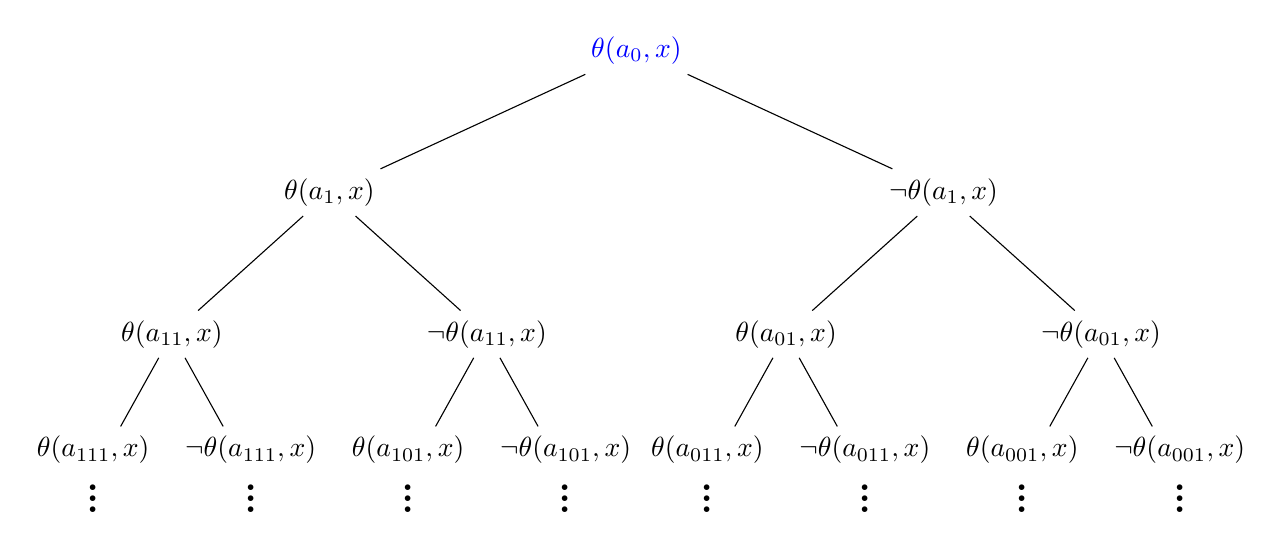
\begin{tikzpicture}[level distance=1.8cm,
level 1/.style={sibling distance=7.8cm},
level 2/.style={sibling distance=4cm},
level 3/.style={sibling distance=2cm}]
\tikzstyle{every node}=[draw=none]

\node (Root) [blue] {$\theta(a_0, x)$}
    child {
    node {$\theta(a_1, x)$} 
    child { node {$\theta(a_{11}, x)$}
    child { node { $\underset{\Huge\vdots}{\theta(a_{111},x)}$  }    }  child { node { $\underset{\Huge\vdots}{\neg{\theta(a_{111},x)}}$ }}}
    child { node {$\neg{\theta(a_{11}, x)}$} child { node { $\underset{\Huge\vdots}{\theta(a_{101},x)}$  }    }  child { node { $\underset{\Huge\vdots}{\neg{\theta(a_{101},x)}}$ }} }
}
child {
    node {$\neg{\theta(a_1, x)}$}
    child { node {$\theta(a_{01}, x)$} 
    child { node { $\underset{\Huge\vdots}{\theta(a_{011},x)}$  }    }  child { node { $\underset{\Huge\vdots}{\neg{\theta(a_{011},x)}}$ }}}
    child { node {$\neg{\theta(a_{01}, x)}$} 
    child { node { $\underset{\Huge\vdots}{\theta(a_{001},x)}$  }    }  child { node { $\underset{\Huge\vdots}{\neg{\theta(a_{001},x)}}$ }}}
};

\end{tikzpicture}
\] 
with height $\omega$. We call nodes of the form $\theta(a_{\sigma}, x)$ \textit{positive} and those of the form $\neg{\theta(a_{\sigma}, x)}$ \textit{negative}.  Let $U$ denote any branch of \eqref{eqn:tree}. Let $U_p$ denote the set of all strings $\sigma \in 2^{\aleph_0}$ such that $a_{\sigma}$ occurs in a positive node of $U$. Since $U_p$ is countable, it has an upper bound in $\left(2^{\aleph_0}, <\right)$. Since $\left(2^{\aleph_0}, <\right)$  is a complete order and  $2^{\aleph_0}$ is a limit ordinal, it follows that $U_p$ has a supremum $\tau$ in $2^{\aleph_0}$.  By construction of \eqref{eqn:tree}, if $\theta(a_{\sigma}, x)$ is a positive node of $U$ and $\neg{\theta(a_{\sigma'}, x)}$ is a negative one, then $\sigma' > \sigma$. Hence $\tau \leq \sigma'$ for any $\sigma'$ occurring in a negative node of $U$. As a result,  we see that $\A' \models \varphi[a_{\sigma}, b_{\tau}]$ for any node $\varphi$ of $U$.  

\smallskip

Therefore,  every branch of \eqref{eqn:tree} determines a unique $1$-type over $\thh_Y(\A')$ where $$Y \coloneqq \left\{x\in X \mid x \text{ occurs in a node of }\eqref{eqn:tree}\right\}.$$ This shows that $\left\lvert{\S_1^{\A'}(Y)}\right\rvert = 2^{\aleph_0} > \aleph_0$. But \eqref{eqn:tree} has exactly $$\left\lvert{\bigcup_{n\in \omega}2^n}\right\rvert = \aleph_0$$ many nodes, so that $\left\lvert{Y}\right\rvert = \aleph_0$. Hence $\thh(\A)$ is not $\omega$-stable. 

\end{solution}

\bigskip

Informally, an \textit{abstract logic $L$} consists of a set of $L$-sentences together with a satisfaction relation $\models_L$ between structures and $L$-sentences.

\begin{definition}[L\"owenheim-Skolem property]
We say that $L$ has the \textit{L\"owenheim-Skolem property} if any countable satisfiable $L$-theory  has a model of size $\leq \aleph_0$.
\end{definition}

\begin{problem}[7.]
Consider the extension $L(Q_0)$ of first-order logic by the \textit{generalized quantifier} $\exists^{<\omega}$ signifying ``there are finitely many.'' Formally, $$\A \models \left(Q_0{x}\right)\varphi(x) \iff \left\lvert{\left\{a \in \dom(\A) \mid \A \models \varphi[a]\right\}}\right\rvert < \aleph_0.$$ Show that $L(Q_0)$ has the L\"owenheim-Skolem property.
\end{problem}
\begin{solution}
Without loss of generality, consider $L(Q_0)$ with $\exists^{< \omega}$ replaced by $\exists^{\infty} \coloneqq \neg{\exists^{<\omega}}$. We have the following version of the Tarski-Vaught elementary submodel criterion.
\begin{claim}\label{TV}
Let $\B$ be a structure for $L(Q_0)$ and $\A$ be a submodel of $\B$. Suppose that for any formula $\varphi(\bar{x}, y)$ and any $\bar{a}\in \dom(\A)$,
\begin{gather*}
\left\{b\in \dom(\B) \mid \B \models \varphi[\bar{a},b]\right\} \ne \emptyset \implies \left\{b\in \dom(\A) \mid \B \models \varphi[\bar{a},b]\right\} \ne \emptyset 
\\ \left\lvert{\left\{b\in \dom(\B) \mid \B \models \varphi[\bar{a},b]\right\}}\right\rvert \geq \aleph_0 \implies \left\lvert{\left\{b\in \dom(\A) \mid \B \models \varphi[\bar{a},b]\right\}}\right\rvert \geq \aleph_0
\end{gather*} 
Then $\A \preceq_{L(Q_0)} \B$.
\end{claim}
\begin{proof}[Proof sketch]
This is easily proved by induction on the complexity of formulas just as it is for first-order logic.
\end{proof}
Now, suppose that $\Gamma$ is a countable $L(Q_0)$-theory with an infinite model $\M$. It suffices to show that for any $X\subset \dom(\M)$, there is an elementary submodel $\M'$ of $\M$ such that $X\subset \dom(\M')$ and $\left\lvert{\M'}\right\rvert = \left\lvert{X}\right\rvert + \aleph_0$. To this end, inductively construct an $\omega$-sequence
\[
X \coloneqq X_0 \subset X_1 \subset X_2 \subset \cdots
\] of subsets of $\dom(\M)$ such that $\left\lvert{X_i}\right\rvert = \left\lvert{X}\right\rvert + \aleph_0$ for every $i \in \omega$ as follows. Suppose that we have already defined $X_i$ as desired. For every formula  $\varphi(\bar{x}, y)$ and any $\bar{a}\in X_i$, consider the set
\[
F_{\varphi, \bar{a}} \coloneqq \left\{b\in \dom(\M) \mid \M \models \varphi\left[\bar{a}, b\right]\right\} 
.\] By the axiom of choice, we can find a set of the form
\[ \widetilde{F}_{\varphi, \bar{a}} \coloneqq  
 \begin{cases}
 F_{\varphi, \bar{a}}  & F_{\varphi, \bar{a}} \text{ is finite}
 \\ \text{a chosen countably infinite subset of } F_{\varphi, \bar{a}}  & \text{otherwise}
\end{cases}.
\] Now, let 
\[
X_{i+1} = X_i \cup \bigcup_{\varphi, \bar{a}} \widetilde{F}_{\varphi, \bar{a}}.
\] Since there are countably many formulas and, by induction, $ \left\lvert{X}\right\rvert + \aleph_0$ many $\bar{a}\in X_i$, we deduce that $X_{i+1}$ has cardinality $ \left\lvert{X}\right\rvert + \aleph_0$. 

\smallskip 

It is easy to see that the union $\M'\coloneqq \bigcup_{i\in \omega}X_i$ forms an elementary submodel of $\M$ thanks to \cref{TV}. Further, we have that $\left\lvert{\M'}\right\rvert = \left\lvert{X}\right\rvert + \aleph_0 + \aleph_0 =  \left\lvert{X}\right\rvert + \aleph_0$, as desired.
\end{solution}

\medskip

Let $X\subset \omega$. We write $\phi_e^X: W_e^X \to \left\{0,1\right\}$ for the partial function computed by the Turing machine with index $e$ and access to an oracle for $X$. 

\begin{definition}[Computability] Let $Y\subset \omega$.
\be
\item We say that $Y$ is \textit{computable/recursive relative to $X$} if the characteristic function $\chi_Y$ equals $\phi_e^X$ for some index $e$.
\item We say that $Y$ is \textit{computably/recursively enumerable relative to $X$} if $Y= W_e^X$ for some index $e$.
\ee
If $Y= \emptyset$, then we omit ``relative to $X$.''
\end{definition}

Let $\mathcal{C}$ denote any collection of computably enumerable sets. We say that a set $B\subset \left\{0,1\right\}^{\ast}$ of binary strings is a \textit{weak index set for $\mathcal{C}$} if $\mathcal{C} = \left\{W_e \mid e \in B\right\}$. 

\begin{problem}[8.]
Let $\mathsf{REC}$ denote the collection of all recursive sets. Show that $\mathsf{REC}$ has a computably enumerable weak index set.
\end{problem}
\begin{solution}
By mapping all invalid encodings of Turing machines to a distinguished trivial Turing machine, we may assume that our binary representation scheme $$\left\langle{-}\right\rangle : \left\{a \mid a\text{ is a }\TM\right\} \to \left\{0,1\right\}^{\ast}$$ of Turing machines is surjective, i.e., every binary string represents a Turing machine. Therefore, we may computably enumerate all Turing machines 
 \[
M_1 < M_2 < M_3 <\cdots
 \] according to the string order $<$. With this in mind, construct an enumerator  $E$ that prints, for each Turing machine $M_i$, the binary representation of a new Turing machine $M_i'$ given as follows.
 
 \smallskip
 
 \begin{algorithm}[H]
    \SetKwInOut{Input}{Input}
    \Input{the binary string $x$}
    {run $U_{\TM}$ on $\left\langle M_i, x\right\rangle$}\;
         \eIf{$U_{\TM}$ rejects}{reject}{run $U_{\TM}$ on $\left\langle M_i,y\right\rangle$ for all strings $y$ such that $\left\lvert{y}\right\rvert \leq \left\lvert{x}\right\rvert$\;\eIf{$U_{\TM}$ halts for each such $y$}{accept}{reject}}
      \caption{pseudocode describing $M_i'$}
\end{algorithm}
 
 \smallskip
 
Here, $U_{\TM}$ denotes a universal Turing machine. It is easy to see that
 \[
 L(M_i') = \begin{cases}
 L(M_i) & M_i \text{ is total}
 \\ \text{a finite set} & \text{otherwise} 
 \end{cases}.
 \] We claim that the language $\left\{\left\langle M_i'\right\rangle \mid i \in \Z_{\geq 1}\right\}$ enumerated by $E$ is a weak index set for $\mathsf{REC}$, i.e.,  $$\mathsf{REC} = \left\{L(M_i') \mid i \in \Z_{\geq 1}\right\}.$$ Indeed, if $Y$ is recursive, then there is some Turing machine $M_k$ deciding it, in which case $Y = L(M_k) = L(M_k')$. Conversely,  for any language of the form $L(M_k')$, $M_k$ is either total or non-total. If it is total, then $L(M_k') = L(M_k)$ and $L(M_k)$ is recursive. If it is non-total, then $L(M_k')$ is finite and thus recursive.

\bigskip

\begin{remark}
We could \emph{not} have used the set $S\coloneqq \left\{D_1, D_2, D_3, \ldots \right\}$ of all  deciders as our weak index set for $\mathsf{Rec}$, for $S$ is not computably enumerable. Indeed, suppose, toward a contradiction, that $S$ is computably enumerable. Enumerate all binary strings $$w_1 < w_2 < w_3 < \cdots.$$ We now can construct a Turing machine $N$ such that for each integer $i\geq 1$,  $N$ accepts $w_i$ if $D_i$ rejects  it and rejects $w_i$ if $D_i$ accepts it. Then $L(N)$ is a decidable language, but $N\notin S$ by construction, a contradiction.
\end{remark}
\end{solution}

\bigskip

Let $T$ be a countable complete theory. For any $n\in \Z_{\geq 1}$, consider the set $S_n(T)$ of all complete $n$-types of $T$ endowed with the topology generated by all sets of the form
\[
\left[\theta(x_1, \ldots, x_n)\right] \coloneqq \left\{\tau \in S_n(T)\mid  \theta(\bar{x}) \in \tau   \right\}, \ \text{$\quad \theta(\bar{x})$ a formula in the language of $T$}.
\] This is known as the \textit{$n$-th Stone space of $T$}. It is clearly Hausdorff. It is also totally disconnected in the sense that every point in $S_n(T)$ has a clopen neighborhood.

\smallskip

Next, consider the Boolean algebra $$B_n(T)\coloneqq \left\{\left[\theta(x_1, \ldots, x_n)\right]\right\}_{\theta(\bar{x})}$$
with meet $\cap$, join $\cup$, and complement $\left({-}\right)^c$. This is isomorphic to the Boolean algebra of all equivalence classes of the form
$$\left\{\varphi(\bar{x}) \mid T \models \varphi \leftrightarrow \theta\right\}$$ with meet $\land$, join $\vee$, and complement $\neg{}$. 

\begin{theorem}\label{Stonecomp}
The space $S_n(T)$ is compact.
\end{theorem}
\begin{proof}
Recall that a topological space $X$ is compact if and only if every family $\left\{C_i \mid i\in I\right\}$ of closed sets in $X$
with the finite intersection property satisfies $\bigcap_{i\in I}C_i \ne \emptyset$. Suppose that $U\coloneqq \left\{\Gamma_i(\bar{x}) \mid i\in I\right\}$ is any family of closed sets in $S_n(T)$ with the finite intersection property. As all basic open sets in $S_n(T)$ are clopen, each $n$-type $\Gamma_i(\bar{x})$ has the form $\left[\neg{\theta_i(\bar{x})}\right]$. We see that $\left\{\neg{\theta_i(\bar{x})}\mid i\in I\right\}$ is an $n$-type over $T$ because $U$ has the finite intersection property.
\begin{claim}\label{compcon}
Every $n$-type  over $T$ is contained in a complete $n$-type over $T$.
\end{claim}
\begin{proof}
Let $\Delta(\bar{x})$ be an $n$-type over $T$. Let $\bar{c}$ be an $n$-tuple of new constant symbols added to the language of $T$. By definition of  an $n$-type over $T$, the theory $T\cup  \Delta(\bar{c})$ in our expanded language is finitely satisfiable. By the compactness theorem, there is some model $\mathbb{M}$ of $T\cup  \Delta(\bar{c})$. Take the reduct $\mathbb{M}'$ of $\mathbb{M}$ to the language of $L$ and let $\bar{a} = \bar{c}^{\mathbb{M}}$. Then $\mathbb{M}' \models T\cup  \Delta(\bar{a}),$ so that 
\[
\Delta(\bar{x})
\subset
\left\{\psi(\bar{x})\mid \mathbb{M}' \models \psi(\bar{a})\right\},
\] which is a complete $n$-type over $T$.
\end{proof}
By \cref{compcon}, we can find a complete $n$-type $\tau$ over $T$ that contains $\left\{\neg{\theta_i(\bar{x})}\mid i\in I\right\}$. Then $\tau$ must belong to the intersection $\bigcap_{i\in I}\Gamma_i(\bar{x})$.
\end{proof}

\begin{remark}
Our proof of \cref{Stonecomp} reveals why the compactness theorem is so named.
\end{remark}

\pagebreak

\begin{problem}[9.]
Prove that $S_n(T)$ is finite if and only if $B_n(T)$ is finite.
\end{problem}
\begin{solution}
First, suppose that $S_n(T)$  is finite. Every element of $B_n(T)$ is a subset of $S_n(T)$, and thus
$$
\left\lvert{B_n(T)}\right\rvert \leq 2^{\left\lvert{S_n(T)}\right\rvert},$$ which is finite.

\smallskip

Conversely, suppose that $B_n(T)$ is finite. Consider the function $h: S_n(T) \to \P(B_n(T))$ defined by $$\Gamma(\bar{x}) \mapsto \left\{\left[\psi(\bar{x})\right] \mid \psi \in \Gamma\right\}.$$ If $\Gamma(\bar{x})$ and  $\Gamma'(\bar{x})$ are distinct complete $n$-types over $T$, then there is some formula $\theta(\bar{x})$ in the language of $T$ such that $\theta \in \Gamma$ and $\neg{\theta} \in \Gamma'$. Hence $h(\Gamma) \ne h(\Gamma')$, so that $h$ is injective. This implies that $$\left\lvert{S_n(T)}\right\rvert\leq 2^{\left\lvert{B_n(T)}\right\rvert},$$ which is finite.
\end{solution}

\end{document}